%% ================================================================================
\chapter{Method}
\label{ch:method}
%% ================================================================================

\section{Data origin}
\label{sec:Data_origin}
%	-Data origin
%		-Fermi collaboration
%		-LAT
%		-Fermi FTOOLS
%		-point source subtraction
%		-pass7 vs pass8
%			-wider energy range
%			-better statistical and systematic errors
%			-better event selection

\begin{figure}
 \centering
 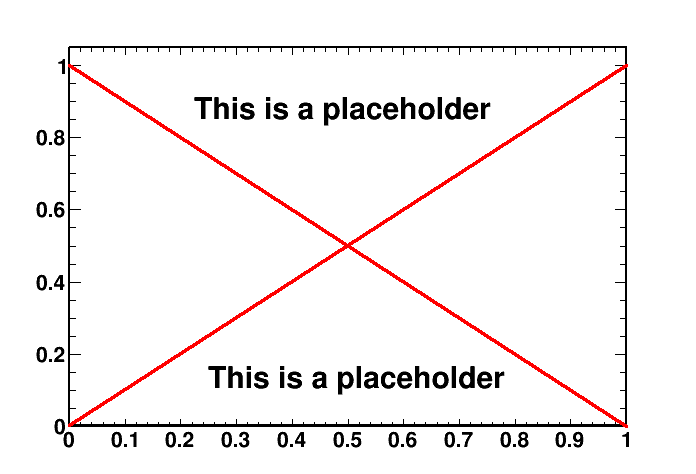
\includegraphics[width=.9\linewidth]{pic/dummy.png}
 \caption{figures of raw data, and after point source subtraction. Maybe also some spectrum with pass7 and pass8 to see the differences.}
 \label{fig:method_pass8}
\end{figure}

The data I used are taken from the Fermi collaboration Large Area Telescope (LAT). They are available on the web and can be treated by anybody using the software given by Fermi.\\

Part of my jobs has been to update the old data we used to use, passing from pass 7 to pass 8. It results in better statistics because of a longer observation period, better systematic errors, wider energy range and better point source subtraction.\\

For our study we are only interested in the diffuse sources of gamma-rays from inside or outside the milky way. The mandatory step to obtain this is to substract the point source emmision from stars, or other direct sources.\\

The Fermi Large Area Telescope Third Source Catalog (3FGL) was used as a reference to subtract the point sources from the raw data. It lists more than 3000 sources and their associated spectra in the 100 MeV-300 GeV range.\\





\section{Model components}
\subsection{Basic components}
%	-3 Basic components
%		-PCR
%			-proton CR follow power-law E^-2.849
%			?-try with break at 5-10GeV with index ~ -2.7 ?
%		-IC and BR
%			-electron CR spectrum E^-3.21
%			-break at 1GeV, index E^-3.21 + 2.4 below break

\subsubsection{$\pi^0$ production by propagated cosmic rays (PCR)}

\begin{figure}
 \centering
 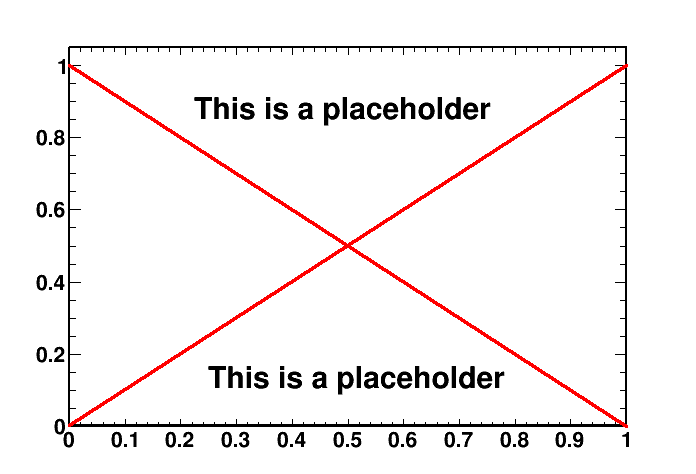
\includegraphics[width=.9\linewidth]{pic/dummy.png}
 \caption{images for proton spectrum for PCR, MCR, SCR, data}
 \label{fig:proton_spec}
\end{figure}

%%% ARTICLE
The initial propagated proton spectrum for the PCR template is obtained from the locally observed proton data from AMS-02 \todo{cite[55]}. A good approximation is an unbroken power law ($R-\alpha$) with a spectral index ($\alpha$) of 2.85 at rigidities above 45 GV. At lower rigidities the data are below the power law because of solar modulation \todo{cite[56]}, as can be seen from Fig. \ref{fig:proton_spec}, where the AMS-02 data are plotted as well. To find the best parametrization a set of broken power laws with a grid of breaks and spectral indices above and below the break was constructed and the optimal parametrization was found by interpolation between the fits with the best test statistic. 
The gamma-ray data are well described by an unbroken power law for the protons with a spectral index ($\alpha$) of 2.85 at all rigidities.\\
%%% ARTICLE

There is also the possibility to introduce a break around a few GeV, to have a slightly harder spectrum at lower energies.\\


\subsubsection{Inverse compton (IC) and bremmstrahlung (BR)}

\begin{figure}
 \centering
 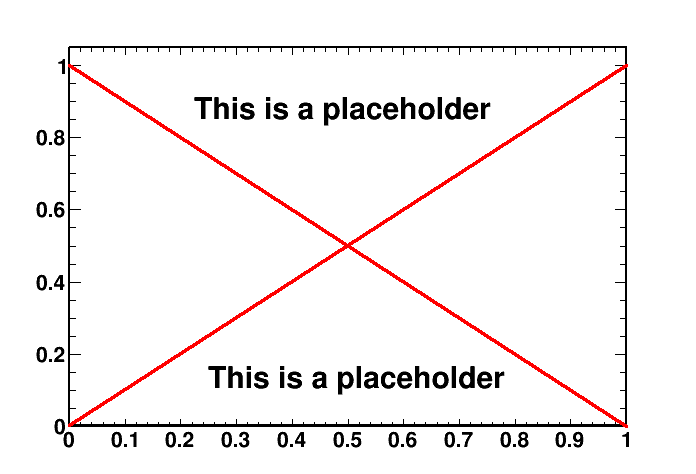
\includegraphics[width=.9\linewidth]{pic/dummy.png}
 \caption{images for electron spectrum for IC, BR, data}
 \label{fig:electron_spec}
\end{figure}
\begin{figure}
 \centering
 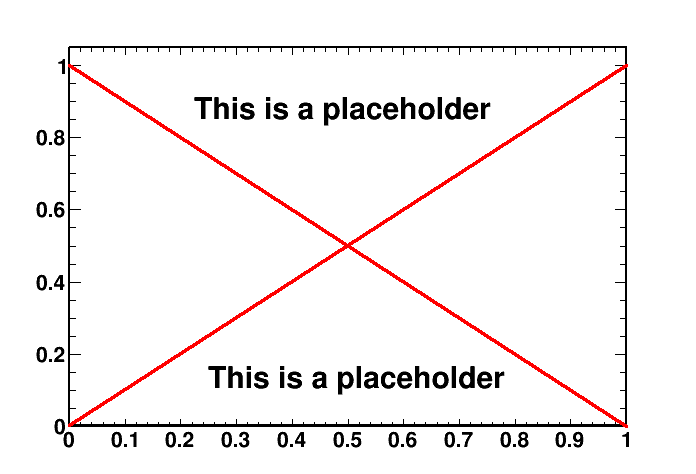
\includegraphics[width=.9\linewidth]{pic/dummy.png}
 \caption{images IC and BR variations over the sky}
 \label{fig:el_variations}
\end{figure}

%%% ARTICLE
The interstellar electron spectra needed a break around \todo{1 GeV} with a spectral index of 3.21 above the break, which is compatible with the locally observed electron spectrum (see Fig. \ref{fig:electron_spec}). Below the break the optimal spectral index is 0.81, which implies a suppression of electrons. The break point might be related to the fact that around 1 GeV electrons have the smallest energy losses, since above this energy synchrotron, BR and IC dominate the energy losses, while below this energy ionization losses become strong, thus depleting the electron spectrum below 1 GeV. A similar break in the electron spectrum was needed in the Fermi diffuse model \todo{cite[46]}.\\
The targets for the production of gamma-rays are the interstellar gas and the interstellar radiation field, which are both stronngly dependant of position, %The latter consists of photons from the cosmic microwave background, the infrared radiation from hot matter, like dust and the star light
, so the photon composition varies with sky direction. 
Hence, for the IC templates we have to calculate the templates for each sky direction. The variation over the sky is about $\pm 10\%$, as shown in \ref{fig:el_variations}; for the BR template the spread is considerably smaller, as shown in \ref{fig:el_variations}. %Note that the intensity of photons in the interstellar radiation field nor the gas density play any role in a template analysis, since the intensity of each contribution to the gamma-ray sky is determined by the fitted normalization factors in Eq. 1.
%%% ARTICLE


%The IC and BR spectra are both obtained from the interstallar electron distribution, taken here as a broken powerlaw with a break \todo{at 1GeV}. The index is 3.21 over the break and 0.8 below.
%The IRF is composed in the mostly by starlight (UV), and in with smaller contribution dust emission (IR) and the cosmic microwave background. The first two components of the IRF are position dependant, and this is why we have to calculate the IC spectrum for every sky direction.
%The BR component is directly linked to the gas, and charged particles distribution. This is also a reason too calculate the BR component in every sky directions. The variations are not too large.




\subsection{Additional components}
%	-2 or more additional components:
%		-SCR
%			-proton CR follow power-law E^-2.1
%		-MCR
%			-proton CR follow power-law E^-2.849
%			-break between 6 and 14GeV, index E^-2.849 + 2.149 below break
%		-DM
%			-Dark Susy
%			-Determination of Mass using best fit in CMZ
%		-MBR
%			-electron CR spectrum E^-3.21
%			-break between 6 and 14 GeV, index E^-3.21 + 2.4 below break
%	-Isosky
%		-Calculated from fermi model and adjusted in our fit

\begin{figure}
 \centering
 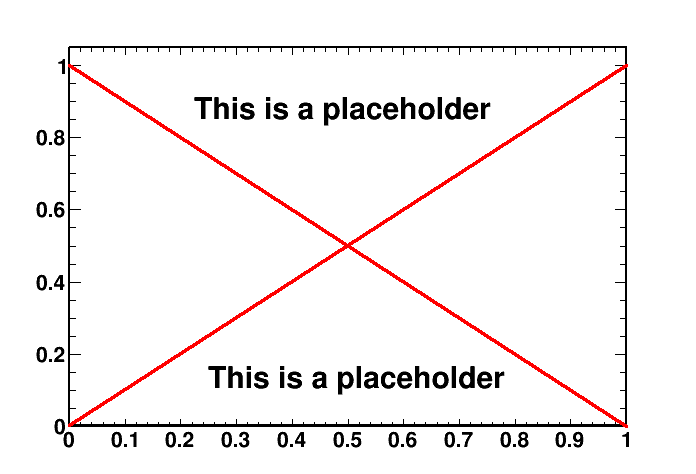
\includegraphics[width=.9\linewidth]{pic/dummy.png}
 \caption{images of MCR, MSP, DM on single plot.}
 \label{fig:excess_component_comp}
\end{figure}

\subsubsection{SCR component}

%%% ARTICLE
The proton spectra for the SCR template can be described by an unbroken power law with a spectral index of 2.1, as obtained from the best fit. The index 2.1 for the SCR template agrees with the data from the Fermi Bubbles, shown by the data points inside the shaded band in Fig. \ref{fig:proton_spec}; the index 2.1 is expected from diffuse shock wave acceleration. \todo{cite[60, 61]} The fact that the Fermi Bubbles and the cosmic rays inside sources have the same spectrum strongly suggests that they are connected by point sources providing advective outflows of gas in the Galactic center. \todo{cite[44]}
%%% ARTICLE

%The proton spectra for the SCR component is a single powerlaw of index 2.1 expecteed from diffuse schock acceleration.

\subsubsection{MCR component}
%%% ARTICLE
The decreasing gamma-ray emissivity from MCs below 2 GeV could be parametrized by a break in the power law of the corresponding proton spectrum. Above the break the optimal spectral index of 2.85 was found to be the same as for the PCR spectrum, as expected if the high energy propagated protons are above a certain magnetic cutoff. But below the break, which varies according to the fit from 6 to 14 GV for the different clouds, the optimal spectral index is 0.7, thus providing a significant suppression of protons below the break, as can be seen from Fig. \ref{fig:electron_spec}. Energy losses alone cannot reproduce such a suppression of the proton spectrum below the break, but magnetic cutoffs are able to do so. Such a cutoff is well known from cosmic rays entering the Earth's magnetic field: particles below typically 20 GV entering near the magnetic equator do not reach the Earth, but are repelled into outer space by the geomagnetic cutoff. \todo{cite[62]} The rigidity cutoff of 20 GV is proportional to the magnetic moment. Although the magnetic field near the Earth (0.5 G) is orders of magnitude higher than the typical magnetic fields in dense MCs \todo{cite[63]}, the much larger sizes of MCs - or its substructure of filaments and cloudlets \todo{cite[64]} - yield magnetic moments of the same order of magnitude as the Earth's magnetic moment, so similar magnetic cutoffs are plausible. Variations in the magnetic cutoff in MCs are expected from the variations in size and in magnetic field; the latter increases with MC density. \todo{cite[63]} The variations of the break in the proton spectrum between 6 and 14 GV varies the maximum of the gamma-ray spectrum from 2 to 1 GeV\todo{??, as shown in Fig. ref??}.
The fit prefers a constant spectral index below the break for all sky directions. Such a constant spectral index is plausible with regular magnetic fields oriented in the disk \todo{cite[65, 66]} and the "cloudlets" inside MCs \todo{cite[64]} form magnetic dipole fields. Then the maximum cutoff occurs for cosmic rays entering from the halo perpendicular into the cloud for any orientation of the magnetic dipole. For a given entrance angle the cutoff would provide a sharp break, but for an isotropic distribution of entrance angles the break points are smeared. A distribution of break points will provide a slope below the maximum break determined largely by the isotropic distribution of the entrance angles into the disk. Since this distribution is the same for all MCs the slopes below the break will be similar for all MCs, even if the maximum break (= maximum magnetic cutoff) varies.
%%% ARTICLE

%
%The MCR component is produced by the same process than for PCR, but with a different proton distribution. Due to the magnetic cut-off in MCs, we introduce a break in the proton spectrum between 6 and 14GeV. We leave the index above to 2.85 as for PCR as expected, but we reduce it to 0.7.\\
%
%The magnetic fields around such clouds are not as strong than what we have in the solar system, but the spatial scales are much bigger and could produce such a break. Of course it position may vary from clouds to clouds and it is why we choose to free its position when fitting.\\
%
%This gives us a spectrum peaking around 2GeV.


\subsubsection{Dark matter (DM)}
%%% ARTICLE
DM particles are expected to annihilate and just like in electron-positron annihilation the annihilation energy of
roughly twice the WIMP mass will lead to the production of hadrons, thus producing copiously gamma-rays from $\pi^0$ decays. A smaller fraction of WIMP annihilation is expected to lead to tau lepton pairs, which can lead to $\pi^0$ production in the hadronic tau decays. This contribution is expected to be small and is neglected. The DM template can be calculated with DarkSusy. \todo{cite[67, 68]} The annihilation signal peaking at 2-3 GeV requires a WIMP mass around 45 GeV, as shown in Fig. \ref{fig:excess_component_comp} as well. The difference to the MCR template is the cutoff at twice the WIMP mass, which is absent in the MCR template.
%%% ARTICLE

%
%The DM spectrum is calculated using the DarkSUSY software. Since the initial WIMP mass is not known, we chose to let the fit decide in the CMZ region and fix it to this value in the other regions. The value generally turns around 50GeV, which make the gamma-ray spectrum peak around 2GeV.


\subsubsection{Milli-second pulsars (MSP)}

The MSP spectrum is directly taken from the Fermi study \todo{cite Fermi}

\subsubsection{Isitropic component}

\begin{figure}
 \centering
 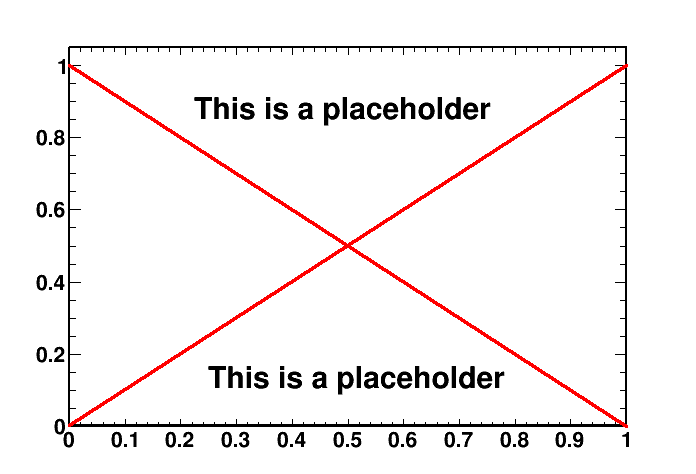
\includegraphics[width=.9\linewidth]{pic/dummy.png}
 \caption{Images to illustrate isotropic calibration}
 \label{fig:iso_calibration}
\end{figure}

%%% ARTICLE
The isotropic template represents the contribution from the isotropic extragalactic background and hadron misiden-tification.  Its spectral shape and absolute normalization are provided within the Fermi software. \todo{cite[51]} The isotropic template was redetermined for our analysis in the following way.\\
We fit the data in regions outside the Bubbles and Galactic disk using the isotropic template from the Fermi software as an initial estimate in the fit. If one plots the total observed gamma-ray flux versus the fitted flux in the various cones in a certain energy bin, one expects a linear relation crossing the origin, if the isotropic flux is estimated correctly. However, if there is a missing or too high isotropic contribution, this leads to an offset at the origin of the linear curve, since the isotropic component is by definition the same for all cones, so it shifts the whole curve up and down for each energy bin. An example of such a fit is shown in Figure \ref{fig:iso_calibration} for an energy bin between \todo{3.7-5.2 GeV}. The offset can be determined for each energy bin, which yields the spectral template of the isotropic component. The final spectral template is obtained by iteration until zero offset at the origin is reached. The resulting template in our analysis has deviations from the Fermi template up to $35\%$ above 2 GeV, as shown in the insert of \ref{fig:iso_calibration}.
%%% ARTICLE

\section{Fitting method}
%My method:
%	-Spectral templates fitted to the data
%		-independant spatial cones on the entire sky (usually 797 for optimized sizes)
%		-minimum chi2 fit using ROOT for every cone
%		-Benefits
%			-energy related features
%			-only a few degrees of freedom -> Well constrained fit (5(or 6) dof against 21-30 points)
%		-Downside:
%			-No spatial templates. (only the isosky)


The fitted data can be seen as a data cube whose dimension are longitude, latitude and energy. The sky is divided in $720\times360$ cones of $ 0.5^\circ \times 0.5^\circ $. Every cone contains 30 energy bins depending on the data set used. This allows to treat each portion of the sky independently of one another. Since the cones do not have the same solid angle, the grid I will use most often is composed of 797 cones of different sizes whether they are close to the poles or near the equator. This allows a better statistic in lower flux regions at high latitudes. It is also way faster to compute. \\

The model uses a certain number of components (from three to six) each corresponding to a certain phenomenon. They all have a certain energy spectra, that can vary with the position in the sky (for PCR, BR and IC). The fit then only scale every template up and down so that their sum is the closest to the data. The closest is found when the $\chi ^2$ is minimized. The $\chi ^2$ is calculated as follows:

\begin{equation}
\chi ^2 = \sum_{i=1}^{30}[\frac{(D_i - \sum_{j=1}^{n}n_j.T_{ij})^2}{\sigma^2}]
\end{equation}

where:
\begin{itemize}
\item $D_i$ is the data flux in the $i^th$ energy bin.
\item $n_j$ is the scaling factor for the $j^th$ model component.
\item $T_{ij}$ is the model flux of the $j^th$ in the $i^th$ energy bin.
\item $\sigma_i$ is the geometric mean of the statistical and systematical error of the Fermi data point $i$.
\end{itemize}

The fitting routine is executed using the ROOT software. \\

This method allows to fit any region of the sky independently.\\

The fit is also very well constrained with only 5 degrees of freedoms against 30 data points.\\

On the other hand, it is not possible to implement a spatial template where the spatial shape of a component would be fixed in advance. For example a component with a spherical distribution around the GC. The hope is to let the fit find reasonnable shapes by itself only using the $\chi ^2$ minimization.\\

It allows to study at the same time the different contributions in one portion of the sky, and the skymaps of every component.\\



\section{Introduction of results}

Recretion of previous studies (GC excess, problems).\\
Introduction of new component to take care of those problems (SCR for high energies, MCR, Dm or MSP for 2GeV excess)


%%	-Weniger plots
%%		-study of spectra slope between 0.3 and 2 GeV
%%	-Specklings
%%		-Study of symmetry
%%	-Comparison with CO map
